\chapter{Teoría de Control Óptimo}

\section{Planteamiento}
Dado un sistema dinámico:
\begin{align*}
    \dot{x}(t)=f\big( x(t),u(t),t\big) 
\end{align*}
Problema es encontrar $u(t)$, para llevar el estado $x(t)$ hasta $x(t_1)$, para un tiempo finito $t\in[t_0,t_1]$, tal que se cumpla la siguiente condición, donde $J(u)$ es el funcional de desempeño:
\begin{align*}
    J(u)=\int_{t_0}^{t_1}l\big(x(t),u(t),t\big)dt+m\big(x(t_1)\big)
\end{align*}

\begin{itemize}
    \item $\int_{t_0}^{t_1}l\big(x(t),u(t),t\big)dt$: ``Costo de viaje'' (running cost)
    \item $m\big(x(t_1)\big)$: costo terminal
\end{itemize}
El problema de control óptimo se define como:
\begin{align*}
    u^o=\text{arg min}_{u_{[t_0,t_1]}}J(u)
\end{align*}
Se define la \textcolor{red}{función de valor V} como el mínimo costo posible para la trayectoria del sistema dinámico para todos los controles posibles $u_{[t_0,t_1]}$:
\begin{align*}
    V(x_0,t_0) = \min_{u_{[t_0,t_1]}}J(u) = \min\Big\{\int_{t_0}^{t_1}l\big(x(t),u(t),t\big)dt+m\big(x(t_1)\big)  \Big\}
\end{align*}

\section{Principio de Optimalidad}
Para cada $t\in[t_0,t_1)$ y $x\in\mathbb{R}^n$, y para $\Delta t\in[0,t_1-t)$, la función de valor $V(x,t)$ satisface la relación: 

\begin{align*}
    V(x,t) = \min_{u_{[t,t+\Delta t]}} \Big\{ \int_t^{t+\Delta t} l\big(x(s),u(s),s\big)ds+V\big(x(t+\Delta t),t+\Delta t\big)\Big\}
\end{align*}
\begin{itemize}
    \item $\int_t^{t+\Delta t} l\big(x(s),u(s),s\big)ds$: costo asociado al intervalo $[t+\Delta t]$
    \item $V\big(x(t+\Delta t),t+\Delta t\big)$: ``costo a seguir'' mínimo partiendo en $x(t+\Delta t)$ y $t+\Delta t$ $\Longrightarrow$ costo asociado al intervalo $[t+\Delta t,t_1]$
\end{itemize}

\underline{Intuición}: 
\begin{figure}[H]
\centering
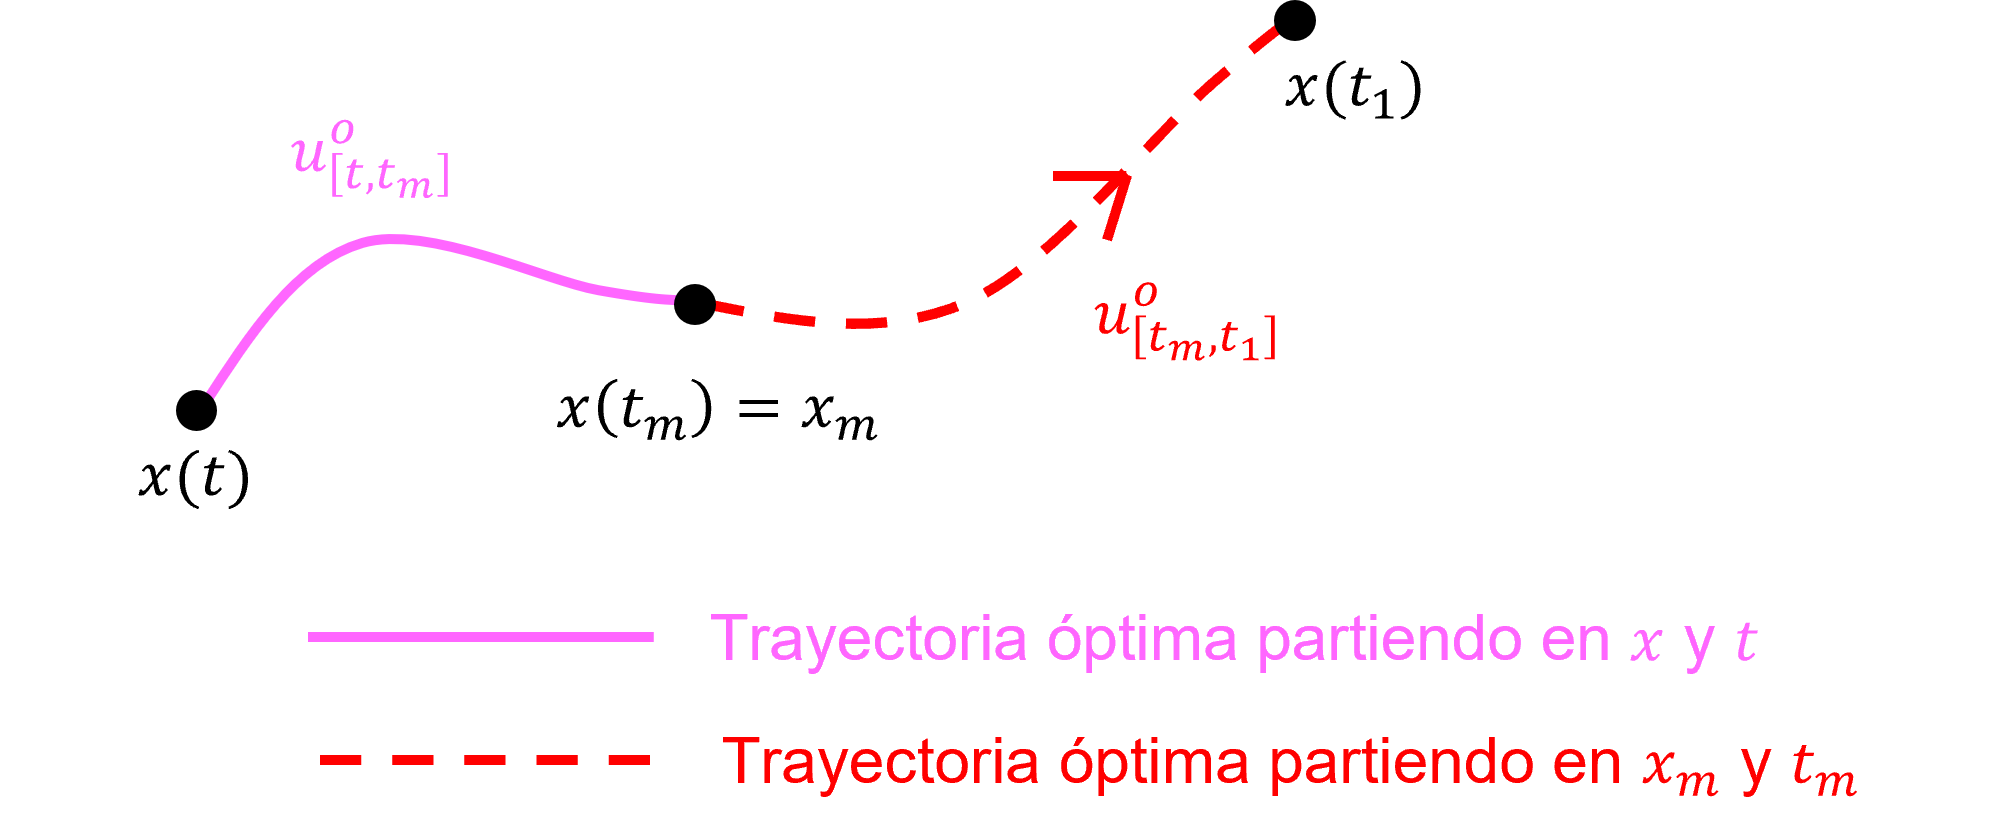
\includegraphics[scale=0.7]{Figuras/optimalidad.png}
\end{figure}

\section{Ecuación HJB (Hamilton-Jacobi-Bellman)}
Esta ecuación resuelve $V(x,t)$ y se obtiene de la siguiente forma:
\begin{enumerate}
    \item Principio de Optimalidad
    \item Realizar una expansión de Taylor de $V(x+\Delta x,t+\Delta t)$ con respecto a $V(x,t)$
    \item Combinar 1. y 2. y dividir por $\Delta t$
    \item Calcular límite para $\Delta t\to 0$
\end{enumerate}

\begin{align*}
    \text{Ec. HJB: } \quad -V_t(x,t) = \min_{u \in \mathcal{U}} \left\{ l(x,u,t) + \left( \nabla_x  V(x,t) \right)^T f(x,u,t) \right\}
\end{align*}

donde $V_t=\frac{\partial V}{\partial t}$, $\nabla_xV=\frac{\partial V}{\partial \tend{x}}$ \\
\par Notar que la ecuación HJB es una ec. diferencial parcial. Por lo tanto, para resolver necesitamos condiciones de borde:
\begin{align*}
    V\big(x(t_1),t_1\big)=m\big(x(t_1)\big)
\end{align*}

\underline{Definición}: Hamiltoniano
\begin{align*}
    H(x,p,u,t) = l(x,u,t)+p^\top (x,t)f(x,u,t)
\end{align*}
donde $p(x,t)=\nabla_x V(x,t)$\\

\par Entonces, la ex. HJB se reduce a:
\begin{align*}
    -V_t(x,t)=\min_{u\in\mathcal{U}}H(x,p,u,t)
\end{align*}
Con estas herramientas, formulamos el siguiente algoritmo para diseñar controladores óptimos:
\begin{enumerate}
    \item Construir el Hamiltoniano
    \item Construir la ec. HJB
    \item Buscar $u^o=\text{arg min}_u H(x,p,u,t)$
    \item Substituir $u^o$ en la expresión HJB
    \begin{align*}
        -V_t=H(x,p,u^o,t)
    \end{align*}
    \item Resolver la ec. dif. parcial para determinar $u^o$
\end{enumerate}

\section{Control LQR (Linear Quadratic Regulator)}
Sea el sistema LTI:
\begin{align*}
    \dot{x}=Ax+Bu=f(x,u)
\end{align*}
y el funcional de desempeño:
\begin{align*}
    J(u)=\int_{t_0}^{t_1}[x^\top Q x+u^\top Ru]dt+x^\top(t_1)Mx(t_1)
\end{align*}
Requisitos: $Q$, $R$, $M$ son matrices definidas positivas y simétricas.\\
\par Utilizando el algoritmo para resolver la ec. HJB:
\begin{enumerate}
    \item[1.] Hamiltoniano:
    \begin{align*}
        H(x,u,V_x,t)=x^\top Qx+u^\top Ru+V^\top_x(Ax+Bu)
    \end{align*}
    \item[3.] Buscar $u^o$: $u^o=\text{arg min}_u H(x,u,V_x,t)$
    \begin{align*}
        \Longrightarrow \frac{\partial H}{\partial u}=0 \Longrightarrow \frac{\partial}{\partial u}[[x^\top Q x+u^\top Ru +V_x^\top(Ax+Bu)]=0\\
        \Longrightarrow 2Ru+B^\top V_x=0\\
        \Longrightarrow u^o=\frac{-1}{2}R^{-1}B^\top V_x(x,t)
    \end{align*}
    \item[2. y 4.] \begin{align*}
        -V_t(x,t) &= H(x,u^o,V_t,t)\\
        \Longrightarrow -V_t &= x^\top Qx+(u^o)^\top Ru^o+V_x^\top (Ax+Bu^o)
    \end{align*} 
    \begin{align}
        \Longrightarrow -V_t &= x^\top Qx-\frac{1}{4}V_x^\top BR^{-1}B^\top V_x+V_x^\top Ax
    \end{align}
\end{enumerate}

Suponga que: $V(x,t)=x^\top P(t)x$, $P(t)\in \mathbb{R}^{n\times n}$, $P^\top (t)=P(t)$, $P(t)\succ 0$
\begin{align*}
    V_t &= x^\top \dot{P}(t)x\\
    V_x &= 2P(t)x
\end{align*}

Sustituyendo en (12):
\begin{align*}
    -x^\top \dot{P}x &= x^\top Qx-\frac{1}{4}(2Px)^\top BR^{-1}B^\top (2Px)+(2Px)^\top Ax\\
    \Longrightarrow -x^\top \dot{P}x &= x^\top\left[Q +PA+A^\top P-P^\top BR^{-1}B^\top P \right]x\\
    \Longrightarrow \dot{P} &= Q +PA+A^\top P-P^\top BR^{-1}B^\top P \quad \text{Ec. diferencial de Riccati}
\end{align*}

Resuelto $P(t)\Longrightarrow V(x,t)=x^\top P(t)x$
\begin{align*}
    V_x(x,t) &= 2P(t)x\\
    \Longrightarrow u^o &= 1\frac{1}{2}R^{-1}B^\top V_x(x,t) = -1\frac{1}{2}R^{-1}B^\top (2P(t)x)\\
    u^o &= -R^{-1}B^\top P(t)x\\
    u^o &= -K(t)x
\end{align*}

donde $K(t)=R^{-1}B^\top P(t) \Longrightarrow$ Control óptimo LQR de horizonte finito (gains variable en el tiempo)
\begin{figure}[H]
\centering
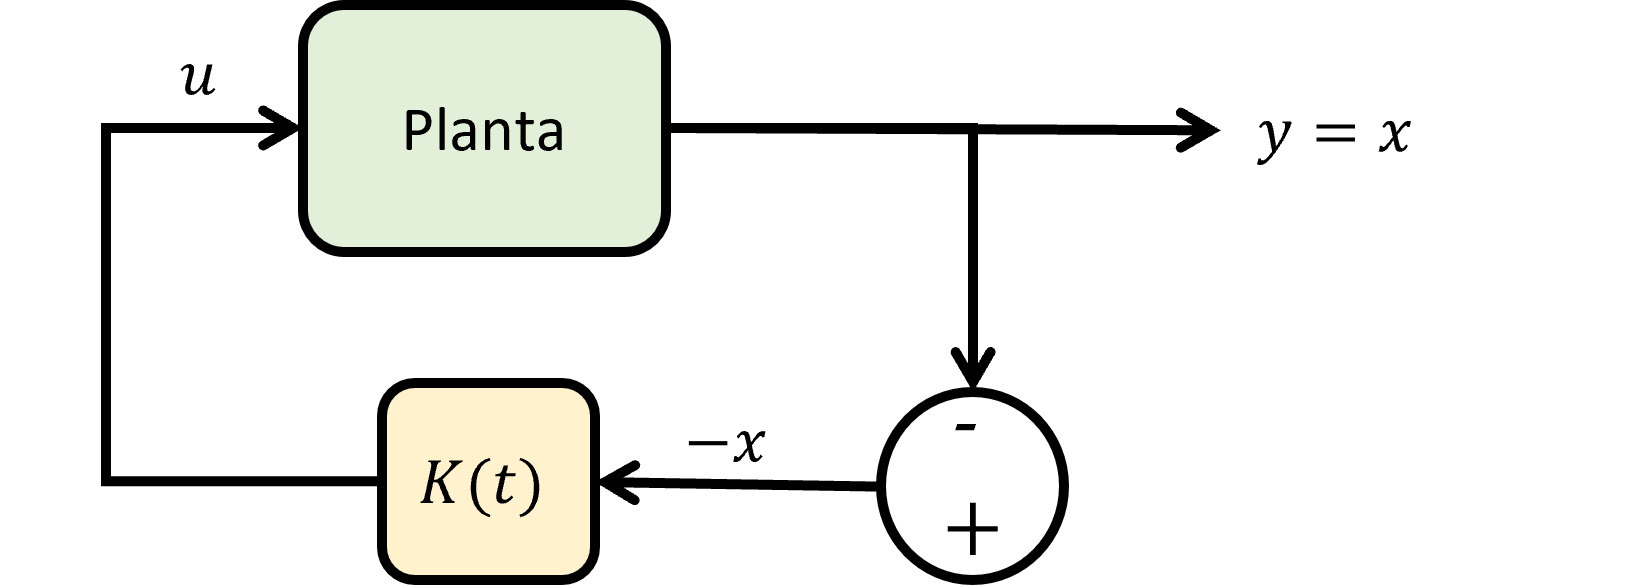
\includegraphics[scale=0.7]{Figuras/LQR.png}
\end{figure}

\section{Control LQR de horizonte infinito}
Dado el sistema LTI: 
\begin{align*}
    \dot{x}=Ax+Bu
\end{align*}
Asumiendo que el sistema es:
\begin{itemize}
    \item estable y controlable, o
    \item inestable, pero los estados inestables son controlables $\Longrightarrow$ estados estabilizables.
\end{itemize}

El problema de control óptimo LQR en horizonte infinito minimiza el siguiente funcional:
\begin{align*}
    J(u) = \lim_{t_1\to \infty} \left[\int_0^{t_1}(x^\top Qx+u^\top Ru)dt \right]
\end{align*}
\underline{Nota}: En este caso, el costo terminal se asume igual a 0.\\
\par Según la lección anterior:
\begin{align*}
    V^{t_1}(x,t)=x^\top P(t,t_1)x \quad \text{: Función de valor para horizonte finito ``$t_1$''}
\end{align*}

Para resolver $P(t,t_1)$, utilizamos la DRE (Differential Riccati Equation):
\begin{align*}
    -\dot{P}=Q+PA+A^\top P-P^\top BR^{-1}B^\top P
\end{align*}
Con condiciones de borde: $P(t_1,t_1)=m(x(t_1))=0$ (costo terminal)\\
\par Finalmente: $u^o(t,t_1)=-R^{-1}B^\top P(t,t_1)x(t)$, con $K(t,t_1)=R^{-1}B^\top$.\\
\par En el límite cuando $t_1\to\infty$, $P(t)$ tiende a una solución de estado estacionario:
\begin{align*}
    \lim_{t_1\to\infty}P(t,t_1)&=P=\text{constante}\\
    \lim_{t_1\to\infty}\dot{P}(t,t_1)&=0
\end{align*}

Entonces, aplicando este supuesto sobre la DRE:
\begin{align*}
    \lim_{t_1\to \infty} \Big[-\dot{P}(t,t_1) &= P(t,t_1)A+A^\top P(t,t_1)+A-P^\top (t,t_1)BR^{-1}B^\top P(t,t_1)  \Big] \\
    \Longrightarrow 0 &= PA+A^\top P+Q-P^\top BR^{-1}B^\top P \quad \text{: Ecuación Algrebaica de Riccati (ARE)}
\end{align*}

Entonces, la función de valor para horizonte infinito:
\begin{align*}
    \hat{V}(x)=x^\top Px
\end{align*}
donde $P$ es la solución de ARE.
\begin{align*}
    \Longrightarrow u^o &= -R^{-1}B^\top Px(t)\\
    &= -K(t)x(t)
\end{align*}
\begin{itemize}
    \item $K=R^{-1}B^\top P$: Gain control LQR horizonte infinito.
\end{itemize}
Finalmente, se puede demostrar que:
\begin{align*}
    V^{t_1}(x,t) \leq J(u)
\end{align*}
\begin{itemize}
    \item $V^{t_1}(x,t)$: Función de valor para horizonte finito $t_1$.
    \item $J(u)$: Funcional de desempeño para horizonte infinito.
\end{itemize}

\subsection{Heurística de diseño}
\par P: ¿Cómo elijo los valores de $Q$ y $R$? 
\par R: Recordar que
\begin{align*}
    J(u) = \int_0^\infty \Big( x^\top Qx+u^\top Ru\Big) dt
\end{align*}
\par Recordar que en sistemas estructurales:
\begin{align*}
    x = \left[
    \begin{array}{c}
     \dot{z} \\ \dot{z} 
    \end{array}\right]
\end{align*}

\begin{itemize}
    \item $z$: desplazamiento
    \item $\dot{z}$: velocidad
\end{itemize}

Podemos escribir la forma cuadrática $x^\top Q x$ de manera tal que le asignamos un significado físico:
\begin{align*}
    \frac{1}{2}x^\top Qx=\frac{1}{2}\left[
    \begin{array}{cc}
     \dot{z} & \dot{z} 
    \end{array}\right] \left[
    \begin{array}{cc}
     K_s & \emptyset \\ \emptyset & M_s 
    \end{array}\right] \left[
    \begin{array}{c}
     \dot{z} \\ \dot{z} 
    \end{array}\right] = \frac{1}{2}z^\top K_s z+\frac{1}{2}\dot{z}^\top M\dot{z}
\end{align*}
\begin{itemize}
    \item $\frac{1}{2}z^\top K_s z$: Energía potencial
    \item $\frac{1}{2}\dot{z}^\top M\dot{z}$: Energía cinética
\end{itemize}

Por otra parte: $u^\top Ru$: energía consumida por el controlador.
\par \underline{Comentario}: No importan los valores absolutos de $Q$ y $R$ en el resultado del control óptimo. Lo que s;i importan son los valores relativos de $Q$ respecto a $R$ (o viceversa).
\begin{align*}
    J(u)=\int_0^\infty (x^\top Qx+u^\top Ru)dt
\end{align*}

\begin{itemize}
    \item $Q$ es mayor que $R$: resultado es sensible a los estados. \\
    \underline{Nota}: Si $R\to 0$: control ``barato'' (cheap) LQR. No es recomendable. \\
    $K=R^{-1}B^\top P$: valor muy grande.
    \item $R$ es mayor que $Q$: resultado es sensible a la señal de control.
\end{itemize}

\subsection{Regla de Bryson}
Elegir $Q$ y $R$ matrices diagonales. Cada componente de $q_{ii}$ y $r_{ii}$ están dados por:
\begin{align*}
    q_{ii} &= \frac{1}{\text{máx valor aceptable de }x_i^2}\\
    r_{ii} &= \frac{1}{\text{máx valor aceptable de }u_i^2}
\end{align*}



\section{Filtro de Kalman (continuo)}
Sea el sistema LTI
\begin{align*}
    \dot{x} &= Ax+B_u u +B_\omega \omega(t)\\
    y &= Cx+v(t)
\end{align*}

donde $\omega$ es la perturbación sobre el sistema y $v$ es el ruido de la medición.\\

\begin{figure}[H]
\centering
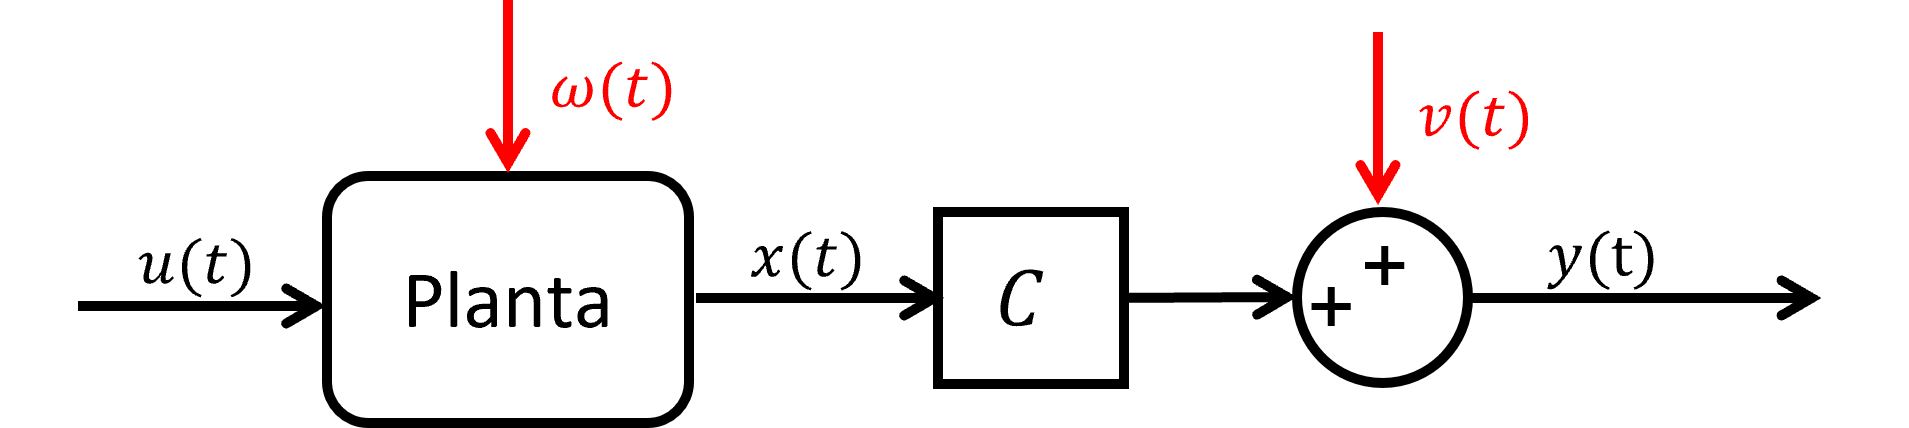
\includegraphics[scale=0.7]{Figuras/wv.png}
\end{figure}

\par \underline{Objetivo}: Estimar los estados $x$ utilizando un observador.\\
\par \underline{Condición}: 
\begin{itemize}
    \item (C,A) es observable
    \item A es Hurwitz
    \item $\Longrightarrow$ Estados detectables
\end{itemize}

Asumir que $\omega (t)$ y $v(t)$ son p.e. Gaussianos, w.s.s., y de media cero:

\begin{itemize}
    \item Perturbación, $\omega (t)$: \begin{itemize}
        \item $\mathbb{E}\{\omega (t)\}=0$
        \item $\mathbb{E}\{\omega (t) \omega^\top (s)\}=Q_\omega \delta(t-s)$
    \end{itemize}
    \item Ruido, $v(t)$: \begin{itemize}
         \item $\mathbb{E}\{v (t)\}=0$
        \item $\mathbb{E}\{v (t) v^\top (s)\}=R_v \delta(t-s)$
    \end{itemize}
\end{itemize}

Asumir en el caso particular que:
$$\mathbb{E}\{\omega(t)v^\top (s)\}=0 \Longrightarrow \text{$\omega(t)$ y $v(t)$ están descorrelacionados} $$

Diseñar un observador óptimo $\Longrightarrow$ Filtro de Kalman.

\begin{figure}[H]
\centering
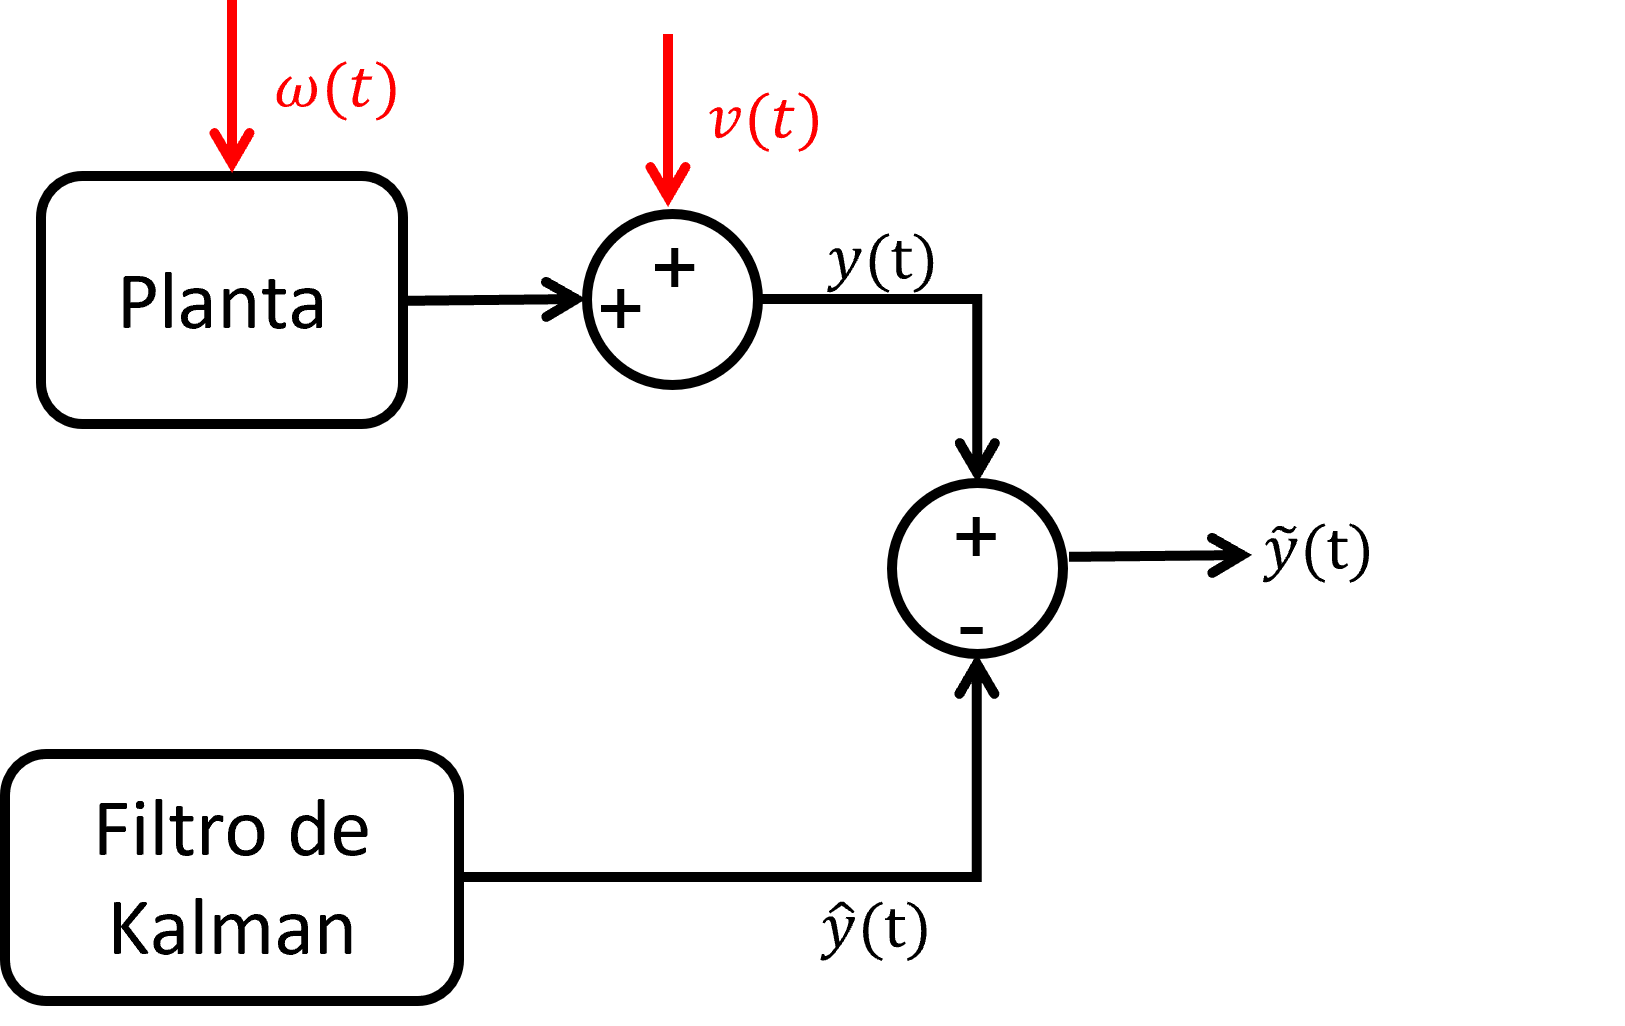
\includegraphics[scale=0.7]{Figuras/Kalman.png}
\end{figure}

\par Problema: 
\begin{align*}
    \text{Minimizar } \tilde{y} &= y-\hat{y}\\
    \Leftrightarrow \text{Minimizar } \tilde{x} &= x-\hat{x}
\end{align*}

\underline{Definición}: Matriz de autocovarianza del error de estado $\tilde{x}$ (en estado estacionario) 

\begin{align*}
    \Gamma=\mathbb{E}\{\tilde{x}\tilde{x}^\top \} \text{: matriz cuadrada, simétrica, definida positiva}
\end{align*}

\underline{Problema}: $\min J$, $J=\text{trace}(\Gamma^\top \Gamma)$
$$J=\mathbb{E} \Bigl\{[x_i-\hat{x}_i][x_i-\hat{x}_i]\Bigr\} $$

Los pasos a seguir son análogos al problema de control óptimo LQR de horizonte infinito. 
\begin{enumerate}
    \item La ganancia de Kalman se define como: $L_{KAL}=\Gamma C^\top R_v ^{-1}$
    \item $\Gamma$ se obtiene de resolver la siguiente ecuación algebraica de Riccati: 
    $$A\Gamma+\Gamma A^\top +\bigl(B_\omega Q_\omega B_\omega^\top -\Gamma C^\top R_v^{-1}C\Gamma\bigr)=0 $$
\end{enumerate}

En términos prácticos, este problema se resuelve en Matlab mediante el comando \texttt{Kalman()}
$$(L_{KAL},\Gamma)=\text{Kalman}(A,C,Q_\omega,R_v) $$

Finalmente:
\begin{align*}
    \dot{\hat{x}} &= A\hat{x}+B_u u+L_{KAL}(y-\hat{y})\\
    \hat{y} &= C\hat{x}
\end{align*}

\begin{figure}[H]
\centering
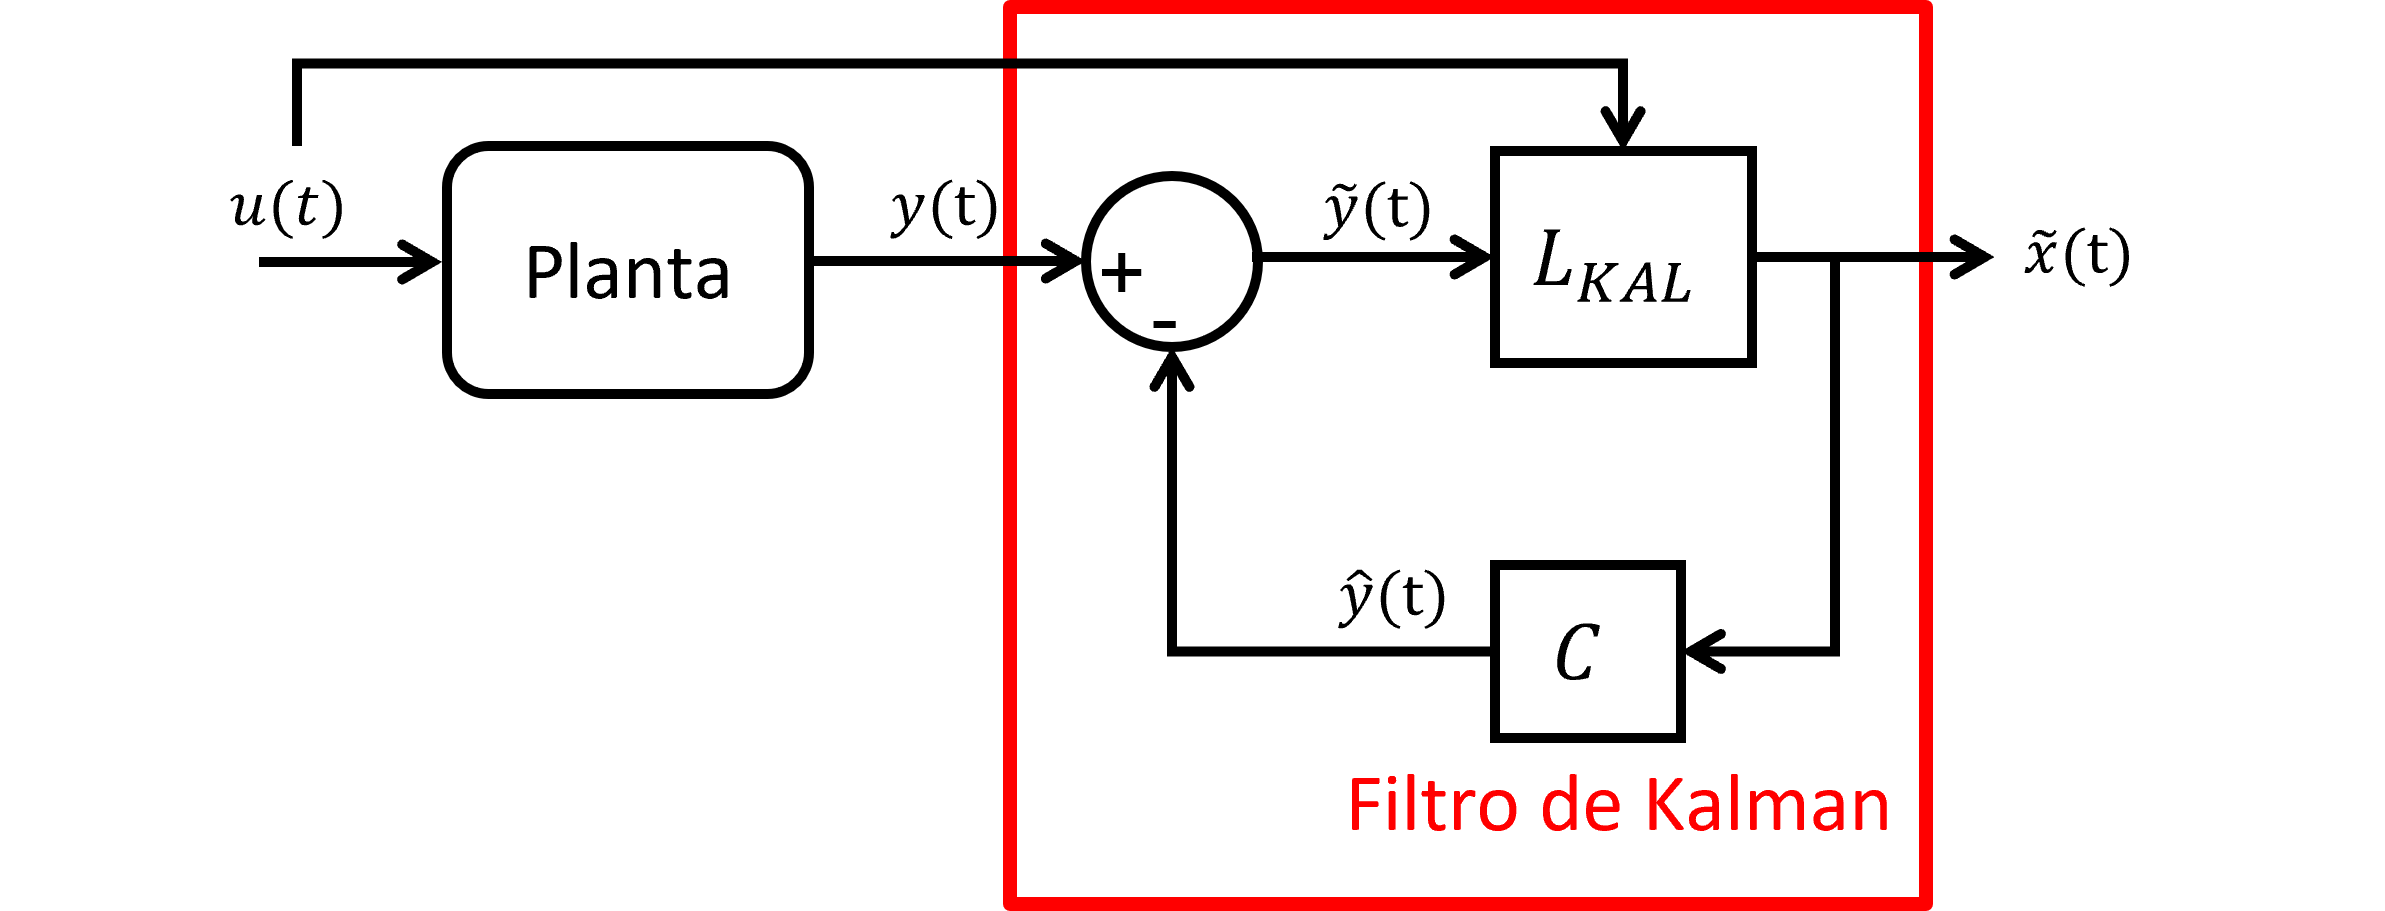
\includegraphics[scale=0.7]{Figuras/Kalman2.png}
\end{figure}

\section{Control LQG}
LQG = Linear Quadratic Gaussian\\
\par Suponga el sistema LTI:
\begin{align*}
    \dot{x} &= Ax+B_u u+B_\omega \omega\\
    y &= Cx+v
\end{align*}

\underline{Objetivo}: diseñar un controlador óptimo con información de la respuesta.

\begin{align*}
    \text{Control óptimo (LQR)} + \text{Obervador óptimo (Kalman)} \overset{\text{Principio de superposición}}{=} LQG
\end{align*}


\begin{figure}[H]
\centering
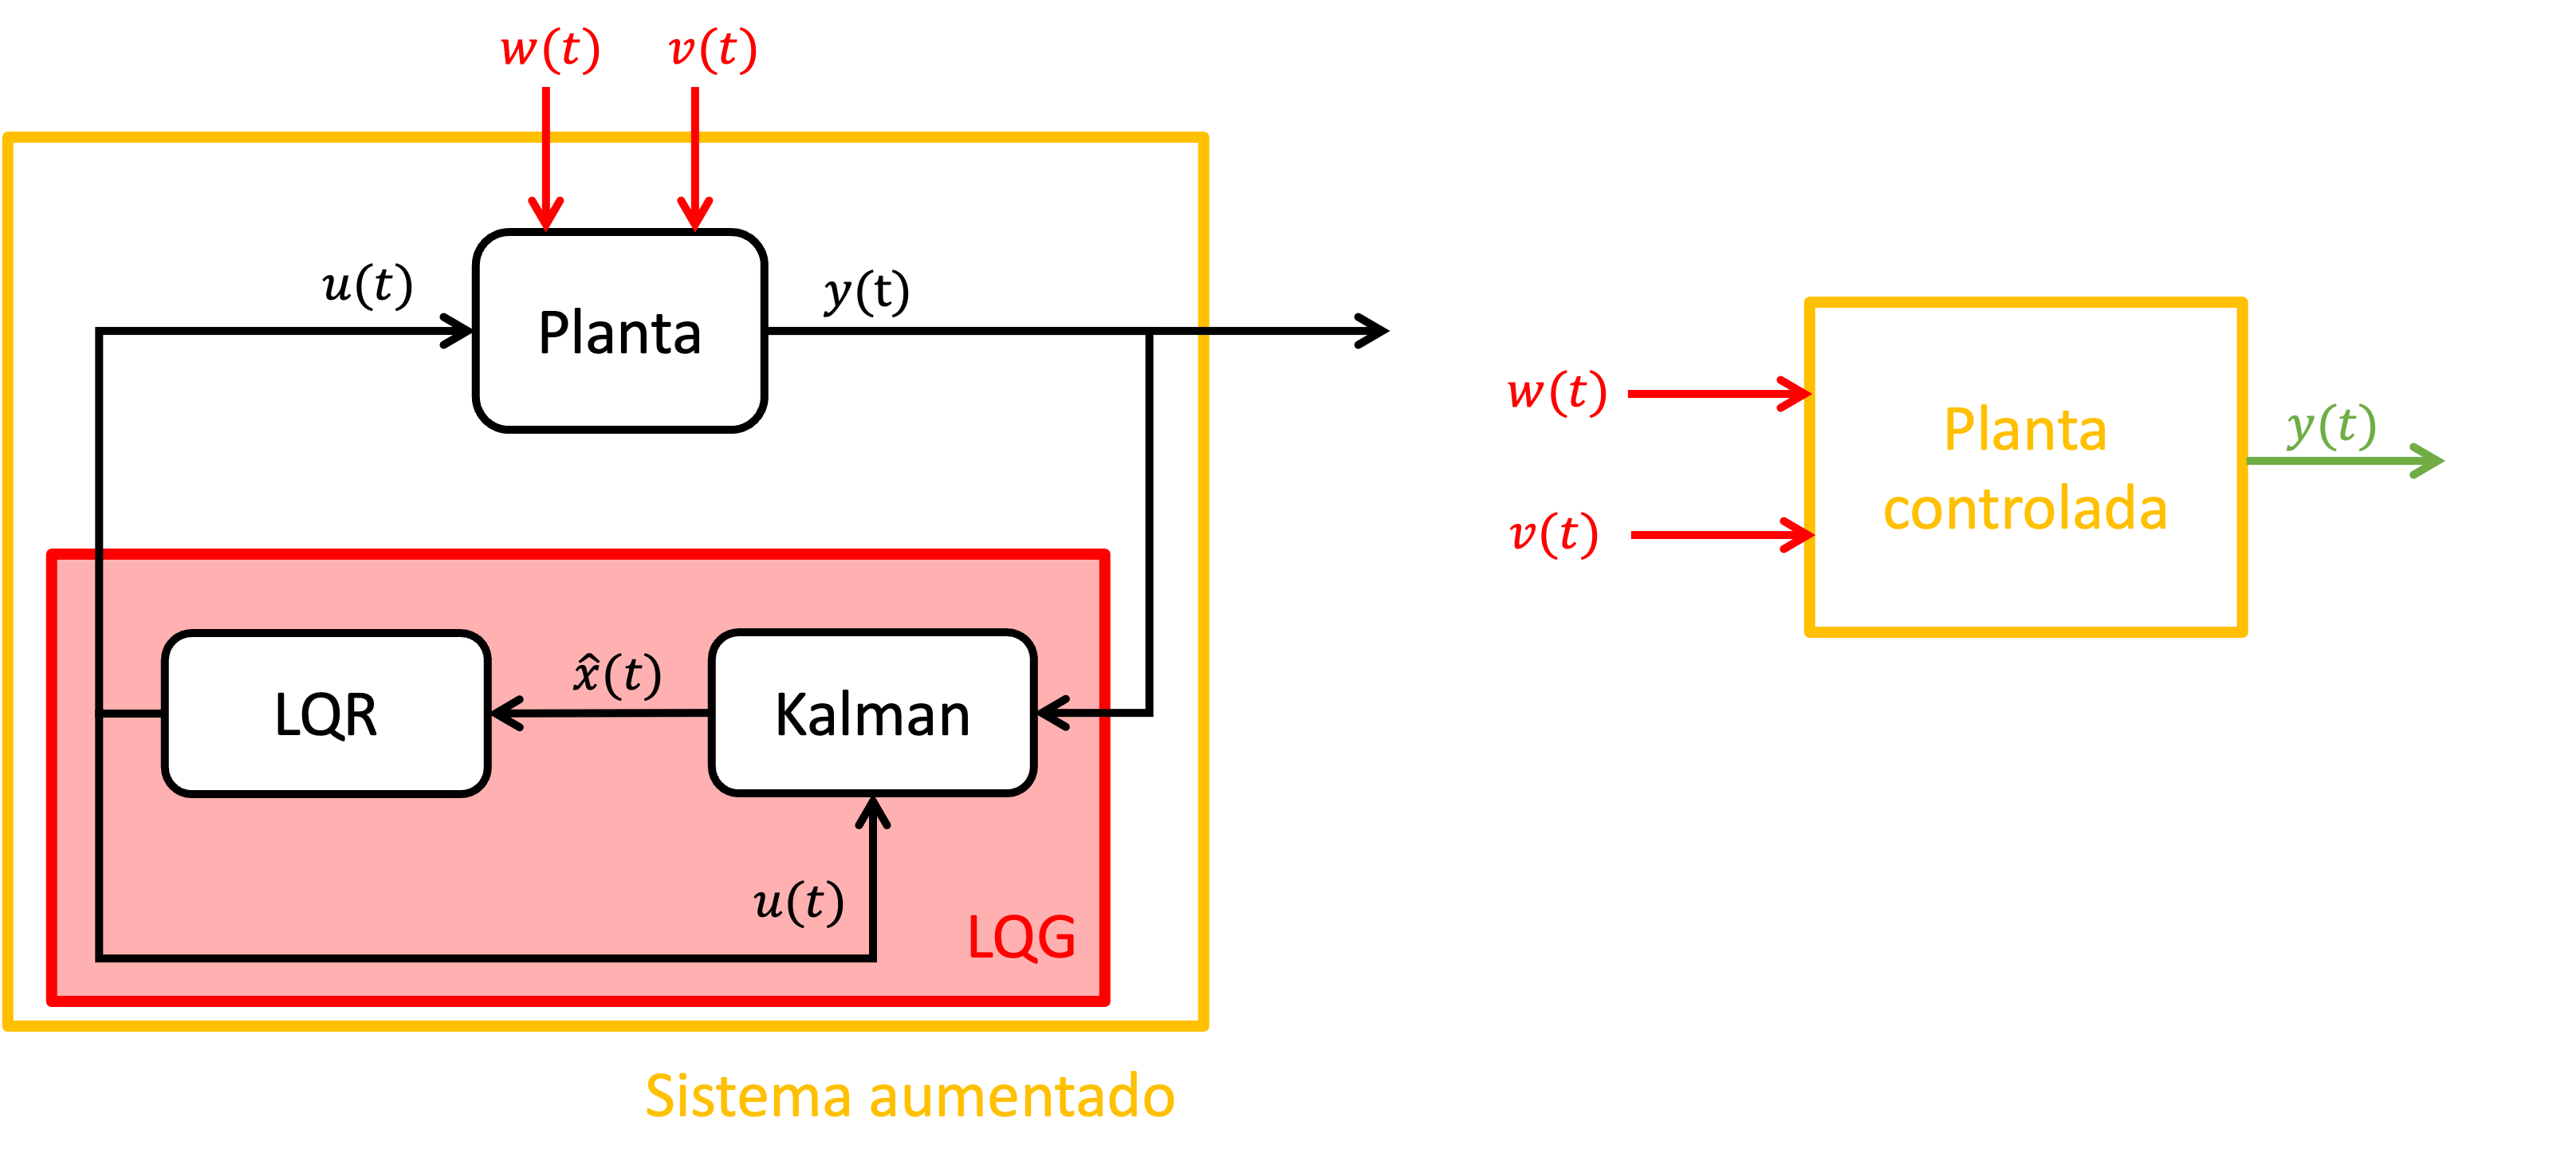
\includegraphics[scale=0.7]{Figuras/LQG.png}
\end{figure}

\underline{Parámetros LQG}: $Q$, $R$, $Q_\omega$, $R_v$.\\


\section{Tópicos especiales en control}

\begin{itemize}
    \item Control robusto (LTR, $H_2$, $H_\infty$, etc.)
    \item Control adaptivo
    \item Control híbrido
    \item Control nolineal
    \item Reinforcement learning
\end{itemize}

